%
% File naaclhlt2015.tex
%


%%%%%%%%%%%%%%%%%%%%%%%%%%%%%%%%%%%%%%%%%%%%%%%%%%%%%%%%%%%%%%%%%%%%%%
% Fix tone, metadiscussion, length
% Finish intro
% Finish summary/future plans
%%%%%%%%%%%%%%%%%%%%%%%%%%%%%%%%%%%%%%%%%%%%%%%%%%%%%%%%%%%%%%%%%%%%%%


\documentclass[11pt,letterpaper]{article}
\usepackage{naaclhlt2015}
\usepackage{times}
\usepackage{latexsym}
\usepackage{enumitem}
\usepackage{graphicx}
\usepackage{float}
\usepackage{array}
\usepackage{booktabs}
\usepackage[table]{xcolor} % http://ctan.org/pkg/xcolor
 \setlength\titlebox{6.5cm}    % Expanding the titlebox

\title{Eye-tracking without the eye-tracker
	% \Thanks{Acknowledgements and thanks go here.}
	}

\author{Authors 1, 2, and 3\\
	Institution\\
	Address Line 1\\
	Address Line 2\\
	{\tt example@college.edu}}

\date{}

\begin{document}
	\maketitle
	\begin{abstract}
		This paper details the process of creating an iPad app for the purpose of measuring eye movements during reading. The app was meant to simulate an eye-tracking experiment as closely as possible without the corresponding equipment. The aim was to replicate established results in the field of text simplification (using eye-tracking equipment) using the app. To this end, a study was designed around minimal sentence pairs, to detect fixations, regressions, and saccades. While we found that the app is capable of detecting small differences in how people process sentences, and there are some statistically significant different phrases amongst the pairs tested, most pairs showed no difference.
	\end{abstract}
	
	\section{Introduction}
	
	In 2015, the U.S. Department of Education and the National Institute of Literacy conducted a study showing that 14\% of adults in the U.S. cannot read beyond a ``basic level'' (``The U.S. Illiteracy Rate''). For the millions of adults that fall within this category, information and resources predicated on reading is difficult to access, leading to issues with daily tasks, ranging from reading the news to acquiring healthcare. A great number of these adults may be unable to read due to learning disabilities, insufficient instruction in school, or not being native English speakers. In all of these cases, it is of vital importance to these people to have available a resource to simplify reading for them, and it is in this vein that automatic text simplification projects have been undertaken.
	
	\subsection{Purpose}
	
	This paper describes a mechanism designed to conduct research in the first step of automatic text simplification: determining what it means for a text to be ``hard.'' Existing literature in this area relies on observing readers' reactions as they read a text, such as through eye-tracking equipment (Ashby \textit{et al.}). Although effective, eye-tracking studies require participants to come to specialized laboratories and put on cumbersome equipment, involving a lot of effort on the part of both the researchers and the participants. If a method can be found that is just as effective, but significantly less cumbersome, much of the research in this field can be simplified, and future research can be undertaken with ease.
	
	\subsection{Background}
	
	The research of interest to this paper has been conducted in the field of eye-tracking experiments to gauge text difficulty. Rather than create models to automatically simplify texts, this research area focuses on using human readers to identify patterns in the way they read, and use this data to estimate what characteristics of a text are easy or difficult. These patterns take on three forms in particular, based on how our eyes move around naturally when reading.
	
	%%% The numbers here refer to Prof Medero's thesis' references
	
	\begin{itemize}[noitemsep]
		\item[1.] \textit{Fixations} refer to the short durations where the eye is fixed on a particular place or word. People usually fixate on few characters, meaning a word may require more than one fixation to be understood. [66]
		\item[2.] \textit{Regressions} occur when readers return to an earlier point in the text in order to reread it, typically due to either having missed something or requiring a reread for clarification. [17]
		\item[3.] \textit{Saccades} are the small jumps that occur between fixations, and are relatively short (10-100 ms, as opposed to fixations of typically 200-250 ms). [27]
	\end{itemize}
	
	The purpose of this experiment was to show that the app being developed was capable of detecting all three of the above behaviors, which would allow this mechanism to be useful in experiments that are like the established eye-tracking technique.
	
	Results from existing eye-tracking experiments also provide the justification for some of the particular texts tested in this experiment. In particular, the paper ``Eye movements of highly skilled and average readers: differential effects of frequency and predictability'' suggests that certain pairs of words produce distinctly different reactions in readers, and that these reactions can be monitored using the three behaviors listed above. They found a statistically significant difference between word pairs where one word was more ``predictable'' than the other, from the context of the same sentence. It is studies such as these which give us an idea of which characteristics of texts may be worth studying.
	
	\section{App}
	
	In order to carry out the study, we designed an iPad app that would allow us to test many different passages and get an idea of whether we could replicate eye-tracking results.
	
%	\subsection{Implementation Details}
	
%	The app developed over the course of this project was built for the iOS mobile operating system. The intended platform was an iPad, due to its screen size, frequency of use for reading, and inbuilt accelerometer. As such, the original implementation of the app was written in the Swift programming language, using the Xcode 6 IDE. During this project, both programming language and IDE were updated in beta to Swift 2.0 and Xcode 7 respectively.
	
	\subsection{Functionality}
	
	In terms of features, this application was designed specifically for this study, and so its functionality is limited to precisely that which was needed for the experiment.
	
	This app was designed with minimalism in mind. For the purposes of this experiment, it was necessary to keep track of individual data sets while preserving the participant's anonymity. To this end, the first function the app supports is the ability to assign an ID number to each set of data readings. This ID number is filled into a text field by the researcher leading the study.
	
	\begin{figure}[H]
		\centering
		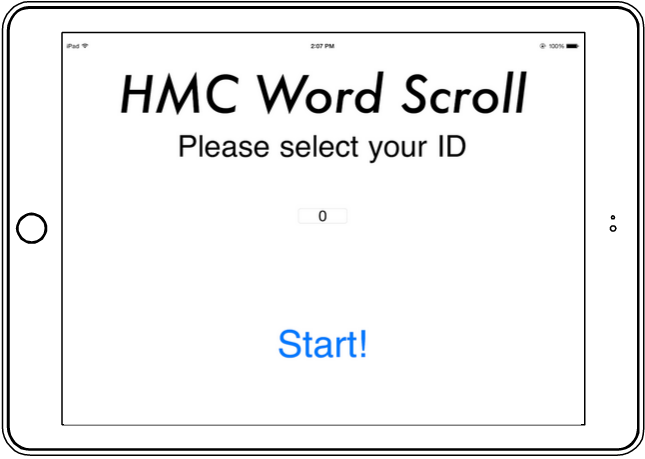
\includegraphics[width=0.4\textwidth]{splashscreen.png}
		\caption{Home screen.}
	\end{figure}
	
	From the home screen, the participant must click ``start" in order to begin the experiment. When this button is pressed, the iPad calibrates itself, meaning whatever position it is held in at that moment is treated as a zero tilt. After this, the user is presented with the reading screen, which consists of a reset button and a horizontal reading frame (a rectangular box in the center of the screen). Upon tilting, text appears inside the reading frame and scrolls through. 
	
	\begin{figure}[H]
		\centering
		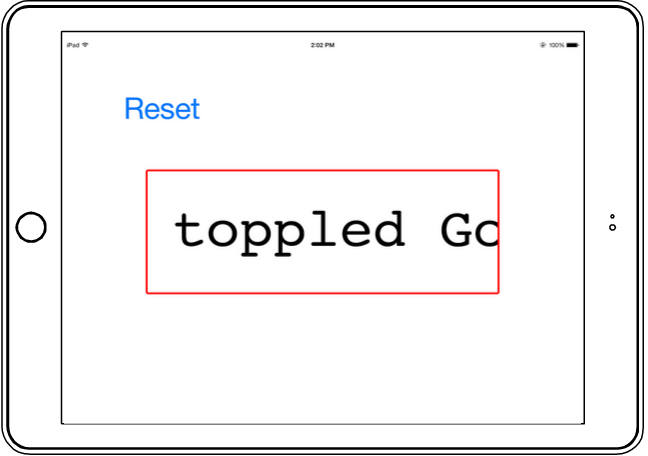
\includegraphics[width=0.4\textwidth]{readingscreen.png}
		\caption{Reading screen.}
	\end{figure}
	
	The accelerometer measures the acceleration as the user tilts the iPad, which is used to determine how fast the text scrolls. The text scrolls from right to left, and the user can make the text scroll forward by tilting the iPad to their right, as well as backward by tilting the iPad to their left. This functionality allows the user to read at their own pace, as well as affords the user the flexibility to reread passages if they so choose.
	
	Many of the settings behind the app were determined through a user study. In the study, participants were given different options for settings for the following parameters:
	\begin{itemize}[noitemsep, nolistsep]
		\item Tilt sensitivity
		\item Reading frame size
		\item Font size
		\item Font choice
		\item Tilt direction
	\end{itemize}
	
	Thus, the above settings were uniform across participants for this text comparison study. Data is collected by the accelerometer built into the iPad, which reads the device's acceleration every 0.2 seconds, and associates this value with the time elapsed and the text visible on the screen at that time.
	
	\section{Experiment}
	\label{sec:exp}
	
	The app was specifically designed for this specific study, which was carried out over the course of three days. Participants were recruited from summer research students, and during the course of the experiment, were asked to read 12 passages. Each passage has an ``A'' and ``B'' version.
	
%	\subsection{Participants}
%	
%	The participants for this study were recruited from amongst summer researchers at Harvey Mudd via email signups. They were told that they would be expected to read a number of passages and summarize them for the researcher leading the study, and that they would be compensated \$5 for their time. Through this recruiting process, the study had 22 participants between the ages of 18 and 22, 10 of whom were female, and 12 male.
%	
%	\subsection{Logistics}
%	
%	Participants were allotted 45 minutes each for the study, although there was no expectation for the study to take over 20 minutes. Each participant began the experiment by reading an informed consent form which explained how the data would be collected, what steps were taken to ensure anonymity, and potential benefits from the study. After signing the form, each participant was given a quick overview of what they were expected to do: they were asked to use the iPad app to read 12 texts back to back, at their own pace, with an emphasis on reading for comprehension. They were given a chance to read a ``test passage," a passage of around 10 words meant to allow users to get used to the controls that had been preset for them. This was in order to avoid recording data that was in reality the user getting used to the given controls.
%	
%	After this test passage, the participant is asked to click the ``Next'' button which appears once a text is complete. For each of the subsequent 12 passages, the participant read the text in silence, and upon completion, summarizes the text briefly for the researcher out loud. We required each participant to summarize each text in order to ensure they were, in fact, reading the passage for comprehension, rather than speeding through the text. Each text the participants read has an ``A'' and a ``B'' version, and a participant reading the ``A'' version of a text does not read the ``B'', and vice versa. The differences between these two versions will be explained in Section 4.3.
%	
%	After reading all 12 passages, the participant was given \$5 as compensation, and asked to sign a form acknowledging receipt of this compensation. If requested, participants were also given a brief explanation of what the texts they read were meant to represent. This information was saved until after the experiment in order to avoid the participants knowing what to expect from the text, as we intended to capture as natural a reading process as possible.
%	
%	The data collected during the participant's reading consists of time values, acceleration values and text indices corresponding to the text on the screen at that time. This data is stored via email.
	
	\subsection{Text Pairs}
	
	The texts used in the experiment were constructed based on sentence pair comparison. The idea behind this technique is as follows: in an effort to identify which aspects of a text are ``easy'' or ``hard'' to read, sentence pairs are constructed, where one sentence serves as control (``B'') and the other as test (``A''). The two sentences differ from each other in small but significant ways. Asking multiple users to read version A, and asking multiple different users to read version B, allows us to compare whether, on average, the differences between A and B had a significant impact on the ``difficulty'' of that passage. Each of the 12 passages the participants read contained three such target sentences, giving us a total of 36 sentence pairs to compare.
	
	There are three kinds of differences that were being tested using the sentence pairs. With four texts for each kind of difference, and each text containing three target sentence, there are 12 sentence pairs per type of difference. These types are as follows.
	
	\textit{Lexical.} A lexical sentence pair consists of two sentences that are identical except for one word. These words must be synonyms of one another, where one of them (the B version) is expected to be more ``difficult'' than the other. An example is given below:
	\begin{itemize}[noitemsep, nolistsep]
		\item[A.] ``... believes that he escapes \textit{liability}... ''
		\item[B.] ``... believes that he escapes \textit{responsibility}... ''
	\end{itemize}
	
	\textit{Semantic.} A semantic sentence pair also consists of two sentences that are identical except for one word. These words are equally correct from a grammatical point of view, but one of them (the B version) is unexpected in the context of the passage, while the other (the A version) must be highly predictable. For instance:
	\begin{itemize}[noitemsep, nolistsep]
		\item[A.] ``... mailed her a \textit{compass} from China... ''
		\item[B.] ``... mailed her a \textit{letter} from China... ''
	\end{itemize}
	
	\textit{Syntactic.} A syntactic sentence pair consists of a garden path sentence (the B version) and another sentence (the A version) which means precisely the same thing as the garden path sentence, but with a clearer syntactic structure. A garden path sentence is one where a reader begins to apply a certain syntactic structure, only to reach a point in the sentence where the structure no longer applies. The addition of some qualifiers explains the intended syntactic structure. Consider the following:
	\begin{itemize}[noitemsep, nolistsep]
		\item[A.] ``The horse raced past the barn \textit{fell}.''
		\item[B.] ``The horse \textit{which was} raced past the barn fell.''
	\end{itemize}
	
% For some reason, the table spanning two columns setting also puts the table on the next page
% So I have moved the code here, and then it should be on top of the following page, where it should be
	
	\begin{table*}[t]
		\begin{center}
			\begin{tabular}{*7c}
				\toprule
				 & \multicolumn{2}{c}{\textbf{Lexical}} & \multicolumn{2}{c}{\textbf{Semantic}} & \multicolumn{2}{c}{\textbf{Syntactic}} \\
				\midrule
				\textbf{Text Number} & A & B & A & B & A & B \\
				1 & $ 0.6306 $ & $ 0.3272 $ & $ 1.1324 $ & $ 0.6256 $ & $-$\textbf{0.2520} & \textbf{0.3485} \\
				2 & $-$\textbf{0.2408} & \textbf{0.4300} & $ 0.4229 $ & $ -0.0737 $ & $ -0.4772 $ & $ -0.4914 $ \\
				3 & \textbf{0.1956} & $-$\textbf{0.8105} & $ -0.1849 $ & $ 0.0549 $ & $ -0.5468 $ & $ -0.1049 $ \\
				4 & $-$\textbf{1.9396} & $-$\textbf{0.8171} & $ 0.1283 $ & $ 0.8202 $ & $ 0.3725 $ & $ 0.0114 $ \\
				\bottomrule
			\end{tabular}
		\end{center}
		\caption{Z-Scores across passages; significant values in bold.}
	\end{table*}
	
	\section{Data Analysis}
	
	\subsection{Acquisition}
	
	Data analysis consisted of two stages, the first run while the app was operational, and the second post-testing. During the operational phase, the indices of the characters on screen were calculated every update step. At this time, the accelerometer reading was converted into characters per second using a linear factor which included the size of each character, the time since last update, and the size of the viewing window. (Note that the size of each character was the same by design, since we chose to use a monospaced font to make such calculations easier.) Thus, each reading yields a time stamp, indices representing the word on screen at that time, and the ``reading speed'' of the user at the time.
	
	\subsection{Processing}
	
	After testing was completed, this data was further analyzed by a separate program. Note that the first five words were discarded in analysis. For each text, the program first gathers all instances of words read by the user; that is, words whose indices had been recorded during the operational phase. Since these values had previously been associated with a characters per second (CPS) value, denoted $x$, the program then uses this data to calculate the average CPS for that particular user across all 12 texts. A second average value was calculated, this time an average ``speed'' for each of the texts, which we denote $\mu_i$, where $i$ represents the text (and ranges from 1 to $n=12$). Finally, the same word can appear on multiple readings, and so have multiple CPS values that correspond to it. An average of all of these values is calculated, denoted $\bar{x}_{i,w}$, representing the average CPS for word $w$ occurring in text $i$.
	
	Each individual word was then scored using the Z-Score, which we denote $S_w$. This calculation used the word's average speed, $\bar{x}_{i,w}$, the average speed of the particular text, $\mu_i$, and the standard deviation of the CPS values fo that text, $\sigma_i$. For instances where a word was truncated, a specific fraction had to be present for the word to be considered ``in-frame." A Z-Score is a measurement of a value's proximity to the mean of the distribution: a Z-Score of 0 implies the value is the same as the mean. This calculation was given by:
	
	\[ S_w = \frac1n \sum_{i=1}^n \frac{\bar{x}_{i,w} - \mu_i}{\sigma_i} \]
	
	Once all users' data had gone through this processing, each word has as many Z-Scores as users that read that particular text. These multiple Z-Scores form a distribution for that particular word, with a corresponding mean and standard deviation. The mean of this distribution provides a normalized score per word across all users. We then compared Z-Score distributions for ``target'' words in the A and B versions of the same text in order to determine whether there was a significant difference (see Results). 
	
	Recall that each pair of texts contains three target words. After completing the above, we considered the Z-Scores of all three words in a passage as a whole. This allows us to get a larger estimation of whether the ``harder'' words were, in fact, more difficult than the easier ones.
	
	
	\section{Results}
	
	By comparing average Z-Scores of partner texts, as described above, we see that only four text pairs showed significant differences in reading speed when run through a T-test for independent samples, with $p < 0.05$  (see Table 1). A higher Z-Score indicates a higher reading speed, and so by comparing the values of A to B, we can see that only three of the four significant pairs support the hypothesis, that the theoretically harder passages would have a lower reading speed across their three target sentences. (Lexical 3 shows a significant difference in the opposite direction from what our hypothesis would suggest.)
	
	\section{Discussion}
	
	\subsection{Summary}
	
	A number of aspects of this experiment were a success. In particular, the data shows that this iPad app is capable of detecting users' reactions to the text they are reading, even relatively small ones. Thus, if there is a signal to be captured, we believe this mechanism can capture it. Further, we found anecdotal support for the hypothesis that the A texts were harder than the B texts, based on comments from participants during the study. There was also some quantitative support for this theory: as discussed in Results, some pairs of texts showed a statistically significant difference in the reaction they produced. 
	
	However, these results were not as numerous or as significant as we had hoped. We believe there are a number of reasons for this. A primary reason could be the randomness in users' behavior. It is possible that we did not stress the importance of accounting for their every reaction to the participants of the study, so some of them were confused by the ``difficult'' words, but did not think it important to pause and let the iPad record that reaction. This led to a random distribution of reactions, which we think explains the lack of statistically significant differences. In order to combat this, we believe a clearer approach needs to be implemented: clarify the goals of the project to the participants, but do not give away enough to affect the results.
	
	It is also possible that the choice of word pairs were not appropriate to the reading level of our participants. While the original eye-tracking results we incorporated also originated with college students, not all of the sentence pairs represented a large gap in difficulty levels. Thus it is possible that an adjustment of the texts, or recruiting participants from a different population, could produce more statistically significant results.
	
	\subsection{Future Directions}
	
	As the above discussion suggests, we believe our next step should be to recruit different participants and carry out a different study. 
	
%	\section*{Acknowledgments}
%	
%	x
	
	\begin{thebibliography}{}
		
		\bibitem[\protect\citename{{Huffington Post}}2013]{Huff:13}
		{Huffington Post}.
		\newblock 2013.
		\newblock {``The U.S. Illiteracy Rate Hasn't Changed in 10 Years.''}
		\newblock Huffington Post, Web.
		
	\end{thebibliography}
	
\end{document}
